%% bare_conf.tex
%% V1.4b
%% 2015/08/26
%% by Michael Shell
%% See:
%% http://www.michaelshell.org/
%% for current contact information.
%%
%% This is a skeleton file demonstrating the use of IEEEtran.cls
%% (requires IEEEtran.cls version 1.8b or later) with an IEEE
%% conference paper.
%%
%% Support sites:
%% http://www.michaelshell.org/tex/ieeetran/
%% http://www.ctan.org/pkg/ieeetran
%% and
%% http://www.ieee.org/

%%*************************************************************************
%% Legal Notice:
%% This code is offered as-is without any warranty either expressed or
%% implied; without even the implied warranty of MERCHANTABILITY or
%% FITNESS FOR A PARTICULAR PURPOSE! 
%% User assumes all risk.
%% In no event shall the IEEE or any contributor to this code be liable for
%% any damages or losses, including, but not limited to, incidental,
%% consequential, or any other damages, resulting from the use or misuse
%% of any information contained here.
%%
%% All comments are the opinions of their respective authors and are not
%% necessarily endorsed by the IEEE.
%%
%% This work is distributed under the LaTeX Project Public License (LPPL)
%% ( http://www.latex-project.org/ ) version 1.3, and may be freely used,
%% distributed and modified. A copy of the LPPL, version 1.3, is included
%% in the base LaTeX documentation of all distributions of LaTeX released
%% 2003/12/01 or later.
%% Retain all contribution notices and credits.
%% ** Modified files should be clearly indicated as such, including  **
%% ** renaming them and changing author support contact information. **
%%*************************************************************************


% *** Authors should verify (and, if needed, correct) their LaTeX system  ***
% *** with the testflow diagnostic prior to trusting their LaTeX platform ***
% *** with production work. The IEEE's font choices and paper sizes can   ***
% *** trigger bugs that do not appear when using other class files.       ***                          ***
% The testflow support page is at:
% http://www.michaelshell.org/tex/testflow/



\documentclass[conference]{IEEEtran}
% Some Computer Society conferences also require the compsoc mode option,
% but others use the standard conference format.
%
% If IEEEtran.cls has not been installed into the LaTeX system files,
% manually specify the path to it like:
% \documentclass[conference]{../sty/IEEEtran}





% Some very useful LaTeX packages include:
% (uncomment the ones you want to load)


% *** MISC UTILITY PACKAGES ***
%
%\usepackage{ifpdf}
% Heiko Oberdiek's ifpdf.sty is very useful if you need conditional
% compilation based on whether the output is pdf or dvi.
% usage:
% \ifpdf
%   % pdf code
% \else
%   % dvi code
% \fi
% The latest version of ifpdf.sty can be obtained from:
% http://www.ctan.org/pkg/ifpdf
% Also, note that IEEEtran.cls V1.7 and later provides a builtin
% \ifCLASSINFOpdf conditional that works the same way.
% When switching from latex to pdflatex and vice-versa, the compiler may
% have to be run twice to clear warning/error messages.






% *** CITATION PACKAGES ***
%
%\usepackage{cite}
% cite.sty was written by Donald Arseneau
% V1.6 and later of IEEEtran pre-defines the format of the cite.sty package
% \cite{} output to follow that of the IEEE. Loading the cite package will
% result in citation numbers being automatically sorted and properly
% "compressed/ranged". e.g., [1], [9], [2], [7], [5], [6] without using
% cite.sty will become [1], [2], [5]--[7], [9] using cite.sty. cite.sty's
% \cite will automatically add leading space, if needed. Use cite.sty's
% noadjust option (cite.sty V3.8 and later) if you want to turn this off
% such as if a citation ever needs to be enclosed in parenthesis.
% cite.sty is already installed on most LaTeX systems. Be sure and use
% version 5.0 (2009-03-20) and later if using hyperref.sty.
% The latest version can be obtained at:
% http://www.ctan.org/pkg/cite
% The documentation is contained in the cite.sty file itself.






% *** GRAPHICS RELATED PACKAGES ***
%
\ifCLASSINFOpdf
  \usepackage[pdftex]{graphicx}
  % declare the path(s) where your graphic files are
  \graphicspath{{images/}}
  % and their extensions so you won't have to specify these with
  % every instance of \includegraphics
  \DeclareGraphicsExtensions{.pdf}
\else
  % or other class option (dvipsone, dvipdf, if not using dvips). graphicx
  % will default to the driver specified in the system graphics.cfg if no
  % driver is specified.
  % \usepackage[dvips]{graphicx}
  % declare the path(s) where your graphic files are
  % \graphicspath{{../eps/}}
  % and their extensions so you won't have to specify these with
  % every instance of \includegraphics
  % \DeclareGraphicsExtensions{.eps}
\fi
% graphicx was written by David Carlisle and Sebastian Rahtz. It is
% required if you want graphics, photos, etc. graphicx.sty is already
% installed on most LaTeX systems. The latest version and documentation
% can be obtained at: 
% http://www.ctan.org/pkg/graphicx
% Another good source of documentation is "Using Imported Graphics in
% LaTeX2e" by Keith Reckdahl which can be found at:
% http://www.ctan.org/pkg/epslatex
%
% latex, and pdflatex in dvi mode, support graphics in encapsulated
% postscript (.eps) format. pdflatex in pdf mode supports graphics
% in .pdf, .jpeg, .png and .mps (metapost) formats. Users should ensure
% that all non-photo figures use a vector format (.eps, .pdf, .mps) and
% not a bitmapped formats (.jpeg, .png). The IEEE frowns on bitmapped formats
% which can result in "jaggedy"/blurry rendering of lines and letters as
% well as large increases in file sizes.
%
% You can find documentation about the pdfTeX application at:
% http://www.tug.org/applications/pdftex





% *** MATH PACKAGES ***
%
%\usepackage{amsmath}
% A popular package from the American Mathematical Society that provides
% many useful and powerful commands for dealing with mathematics.
%
% Note that the amsmath package sets \interdisplaylinepenalty to 10000
% thus preventing page breaks from occurring within multiline equations. Use:
%\interdisplaylinepenalty=2500
% after loading amsmath to restore such page breaks as IEEEtran.cls normally
% does. amsmath.sty is already installed on most LaTeX systems. The latest
% version and documentation can be obtained at:
% http://www.ctan.org/pkg/amsmath





% *** SPECIALIZED LIST PACKAGES ***
%
%\usepackage{algorithmic}
% algorithmic.sty was written by Peter Williams and Rogerio Brito.
% This package provides an algorithmic environment fo describing algorithms.
% You can use the algorithmic environment in-text or within a figure
% environment to provide for a floating algorithm. Do NOT use the algorithm
% floating environment provided by algorithm.sty (by the same authors) or
% algorithm2e.sty (by Christophe Fiorio) as the IEEE does not use dedicated
% algorithm float types and packages that provide these will not provide
% correct IEEE style captions. The latest version and documentation of
% algorithmic.sty can be obtained at:
% http://www.ctan.org/pkg/algorithms
% Also of interest may be the (relatively newer and more customizable)
% algorithmicx.sty package by Szasz Janos:
% http://www.ctan.org/pkg/algorithmicx




% *** ALIGNMENT PACKAGES ***
%
%\usepackage{array}
% Frank Mittelbach's and David Carlisle's array.sty patches and improves
% the standard LaTeX2e array and tabular environments to provide better
% appearance and additional user controls. As the default LaTeX2e table
% generation code is lacking to the point of almost being broken with
% respect to the quality of the end results, all users are strongly
% advised to use an enhanced (at the very least that provided by array.sty)
% set of table tools. array.sty is already installed on most systems. The
% latest version and documentation can be obtained at:
% http://www.ctan.org/pkg/array


% IEEEtran contains the IEEEeqnarray family of commands that can be used to
% generate multiline equations as well as matrices, tables, etc., of high
% quality.




% *** SUBFIGURE PACKAGES ***
%\ifCLASSOPTIONcompsoc
\usepackage[caption=false,font=normalsize,labelfont=sf,textfont=sf]{subfig}
%\else
%  \usepackage[caption=false,font=footnotesize]{subfig}
%\fi
% subfig.sty, written by Steven Douglas Cochran, is the modern replacement
% for subfigure.sty, the latter of which is no longer maintained and is
% incompatible with some LaTeX packages including fixltx2e. However,
% subfig.sty requires and automatically loads Axel Sommerfeldt's caption.sty
% which will override IEEEtran.cls' handling of captions and this will result
% in non-IEEE style figure/table captions. To prevent this problem, be sure
% and invoke subfig.sty's "caption=false" package option (available since
% subfig.sty version 1.3, 2005/06/28) as this is will preserve IEEEtran.cls
% handling of captions.
% Note that the Computer Society format requires a larger sans serif font
% than the serif footnote size font used in traditional IEEE formatting
% and thus the need to invoke different subfig.sty package options depending
% on whether compsoc mode has been enabled.
%
% The latest version and documentation of subfig.sty can be obtained at:
% http://www.ctan.org/pkg/subfig




% *** FLOAT PACKAGES ***
%
%\usepackage{fixltx2e}
% fixltx2e, the successor to the earlier fix2col.sty, was written by
% Frank Mittelbach and David Carlisle. This package corrects a few problems
% in the LaTeX2e kernel, the most notable of which is that in current
% LaTeX2e releases, the ordering of single and double column floats is not
% guaranteed to be preserved. Thus, an unpatched LaTeX2e can allow a
% single column figure to be placed prior to an earlier double column
% figure.
% Be aware that LaTeX2e kernels dated 2015 and later have fixltx2e.sty's
% corrections already built into the system in which case a warning will
% be issued if an attempt is made to load fixltx2e.sty as it is no longer
% needed.
% The latest version and documentation can be found at:
% http://www.ctan.org/pkg/fixltx2e


%\usepackage{stfloats}
% stfloats.sty was written by Sigitas Tolusis. This package gives LaTeX2e
% the ability to do double column floats at the bottom of the page as well
% as the top. (e.g., "\begin{figure*}[!b]" is not normally possible in
% LaTeX2e). It also provides a command:
%\fnbelowfloat
% to enable the placement of footnotes below bottom floats (the standard
% LaTeX2e kernel puts them above bottom floats). This is an invasive package
% which rewrites many portions of the LaTeX2e float routines. It may not work
% with other packages that modify the LaTeX2e float routines. The latest
% version and documentation can be obtained at:
% http://www.ctan.org/pkg/stfloats
% Do not use the stfloats baselinefloat ability as the IEEE does not allow
% \baselineskip to stretch. Authors submitting work to the IEEE should note
% that the IEEE rarely uses double column equations and that authors should try
% to avoid such use. Do not be tempted to use the cuted.sty or midfloat.sty
% packages (also by Sigitas Tolusis) as the IEEE does not format its papers in
% such ways.
% Do not attempt to use stfloats with fixltx2e as they are incompatible.
% Instead, use Morten Hogholm'a dblfloatfix which combines the features
% of both fixltx2e and stfloats:
%
% \usepackage{dblfloatfix}
% The latest version can be found at:
% http://www.ctan.org/pkg/dblfloatfix




% *** PDF, URL AND HYPERLINK PACKAGES ***
%
%\usepackage{url}
% url.sty was written by Donald Arseneau. It provides better support for
% handling and breaking URLs. url.sty is already installed on most LaTeX
% systems. The latest version and documentation can be obtained at:
% http://www.ctan.org/pkg/url
% Basically, \url{my_url_here}.




% *** Do not adjust lengths that control margins, column widths, etc. ***
% *** Do not use packages that alter fonts (such as pslatex).         ***
% There should be no need to do such things with IEEEtran.cls V1.6 and later.
% (Unless specifically asked to do so by the journal or conference you plan
% to submit to, of course. )

\usepackage{flushend} % Balances columns on the last page.
\usepackage{hyperref} % for autoref
\usepackage{amsthm} % for proofs
\usepackage{amsmath} % theorems, definitions, etc.
\usepackage{mathtools} % ::= \Coloneqq
\usepackage{amssymb} % \mathbb
\newtheorem{definition}{Definition}
\newcommand{\definitionautorefname}{Definition}

\usepackage{glossaries}

\newacronym{mde}{MDE}{Model-driven engineering}
\newacronym{bpmn}{BPMN}{Business Process Modeling Notation}
\newacronym{ct}{CT}{category theory}
\newacronym{uml}{UML}{Unified Modeling Language}
\newacronym{dsl}{DSL}{Domain Specific Language}
\newacronym{csp}{CSP}{Communication Sequential Processes}

% correct bad hyphenation here
\hyphenation{be-ha-vi-o-ral}


\begin{document}
\title{Towards behavioral consistency \\ in heterogeneous modeling scenarios}

\author{\IEEEauthorblockN{Tim Kräuter}
\IEEEauthorblockA{Høgskulen på Vestlandet\\
Bergen, Norway\\
Email: tkra@hvl.no}}


\maketitle

% As a general rule, do not put math, special symbols or citations
% in the abstract
\begin{abstract}
Behavioral models play an essential role in \gls{mde}.
Keeping inter-related behavioral models consistent is critical to use them successfully in \gls{mde}. 
However, consistency checking for behavioral models, especially in a heterogeneous scenario, is limited.

We propose a methodology to integrate heterogeneous behavioral models to achieve consistency checking in broader scenarios.
It is based on aligning the respective behavioral metamodels by defining possible inter-model relations which carry behavioral meaning.
Converting the models and their relations to a behavioral formalism enables analysis of global behavioral consistency using model-checking. 
\end{abstract}

% no keywords

\IEEEpeerreviewmaketitle



\section{Problem}
A significant motivation for \glsfirst{mde} is to handle the increasing complexity of software systems by a clear separation of concerns \cite{franceModeldrivenDevelopmentComplex2007}.
In the multi-view modeling approach, a set of models is developed for the different aspects of a system.
Consequently, it is likely that separate groups of people work independently on different parts of the system.
However, this separation of concerns causes problems because models must be kept consistent, i.e., they should not contain contradicting information \cite{cicchettiMultiviewApproachesSoftware2019}.
% mde will fail if the underlying models are inconsistent!
Without this inter-model consistency, \gls{mde} cannot deliver on the promised productivity increase and error reduction \cite{brambillaModeldrivenSoftwareEngineering2017}.

% mde is heterogeneous and has to be kept consistent.
Inter-model consistency is especially problematic when the used models are heterogeneous:
Firstly, structural models such as class diagrams and entity-relationship diagrams exist.
Secondly, behavioral diagrams are used to describe the dynamics of a system.
Widely used diagrams or formalisms for specifying behavior are state machines, activity diagrams, Petri nets, and process algebras.

% We already deal with structural models/ consistency
Inter-model consistency for structural models has been researched extensively.
One promising approach is model weaving \cite{bezivinCanonicalSchemeModel2006}, which establishes links between models with the goal of automatic consistency checking.
Typically, these inter-relations focus on structural aspects, such as identity, usage, dependency, and refinement \cite{feldmannManagingIntermodelInconsistencies2019, torresSystematicLiteratureReview2020}.
They are called \textit{correspondences} on the metamodel level and \textit{commonalities} on the model level \cite{stunkelMultipleModelSynchronization2020, klareCommonalitiesPreservingConsistency2019}.
Inter-model constraints can then be defined and automatically be checked.
This works by either merging individual models to a global model using commonalities \cite{stunkelMultimodelCorrespondenceIntermodel2018} or establishing a comprehensive view of the global model \cite{stunkelMultipleModelSynchronization2020}.

% We have to deal with behavioral/semantic consistency between behavioral models especially of heterogeneous nature
However, there is no general approach to check global behavioral consistency on a collection of models, sometimes called semantic consistency.
% Definition attempt (does not cover dead- and livelocks only simple reaches not reaches.): We define behavioral consistency as the absence of behavioral inconsistency, while behavioral inconsistency means that a collection of behavioral models can reach a combined state with contradicting information or cannot reach a set of desired combined states.
Behavioral models describing interacting parts of a system should be checked for deadlocks, live-locks, and other system-specific requirements.
This is generally not problematic if the models conform to the same formalism or modeling language.
Nevertheless, in a heterogeneous case, one still wants to define interactions between the models and check behavioral consistency.

Using only one formalism or modeling language for behavioral models is not feasible since one wants to use the most suitable formalism or modeling language in each situation.
The modeling formalisms used in each case depend on the system requirements, existing software landscape, and the knowledge and preferences of the responsible developers. 

% We have to deal with consistency between structural and behavioral models in the future as well. Since structural models are graphs, graph transformations seem promising to integrate this in the future.
There can also be consistency rules spanning structural and behavioral models.
For example, messages to objects in a \gls{uml} sequence diagram must match the corresponding classes methods in a class diagram \cite{egyedFixingInconsistenciesUML2007}.
We will focus on behavioral consistency before addressing consistency between structural and behavioral models in future work. 

\section{Related work}
% Engels
\cite{engelsMethodologySpecifyingAnalyzing2001} investigates the consistency of object-oriented behavioral models formulated as capsule statecharts in \gls{uml}-RT.
Consequently, they deal with a homogeneous modeling environment where all behavioral models are developed in the same modeling language.
The authors use the term semantic consistency instead of behavioral consistency.
To check behavioral consistency, they map statechart models to \gls{csp}.
Using the well-defined semantics of \gls{csp}, they validate deadlock freeness and the processes compliance to a previously defined communication protocol.
Their proposed general methodology to analyze consistency is to find a suitable semantic domain and map the models into it.
The semantic domain can then be exploited to check the consistency.

Based on this methodology, consistency checking for sequence diagrams and statecharts was developed in \cite{kusterExplicitBehavioralConsistency2003}.
The consistency requirement claims that all possible interactions specified within sequence diagrams for each class should be possible regarding the behavior of that class defined in a statechart.
As a semantic domain, the authors have successfully used \gls{csp} again.

Besides process algebras such as \gls{csp}, different types of Petri nets are used for behavioral consistency checking.
In \cite{yaoConsistencyCheckingUML2006}, Petri nets were used to check consistency for sequence diagrams and statecharts.
\cite{cunhaFormalVerificationUML2011} analyses sequence diagrams in the context of embedded systems using a transformation to Petri nets.
Consistency for \gls{uml} activity diagrams was checked using Petri nets in \cite{thierry-miegUMLBehavioralConsistency2008}.

All the approaches use model checking to analyze behavioral consistency and follow the methodology defined in \cite{engelsMethodologySpecifyingAnalyzing2001} with variations in the semantic domain.
However, the approaches cover only homogeneous scenarios where all models conform to one modeling language.
An exception is the consistency checking between sequence diagrams and statecharts.
In practice, one could encounter a situation where the combination of state machines, process algebras, Petri nets, and activity diagrams is desired\footnote{The merger of two companies and their IT-infrastructures could for example cause heterogeneity in the used modeling languages.}.
It is possible to check behavioral consistency using our proposed approach even in heterogeneous modeling scenarios.
This leads to more freedom of choice regarding behavioral modeling and model combinations.
In addition, behavioral models of higher quality can be achieved, which lay the foundation for successful and effective \gls{mde}.

\section{Proposed solution}
The proposed solution builds on the methodology presented in \cite{engelsMethodologySpecifyingAnalyzing2001} but introduces a new step inspired by the multi-model consistency management process for structural models defined in \cite{stunkelMultipleModelSynchronization2020}.
The proposed solution can be summarized by the four-step process in \autoref{fig:consistency_process}.
We will explain it in detail now.

\begin{figure}[h]
    \centering
    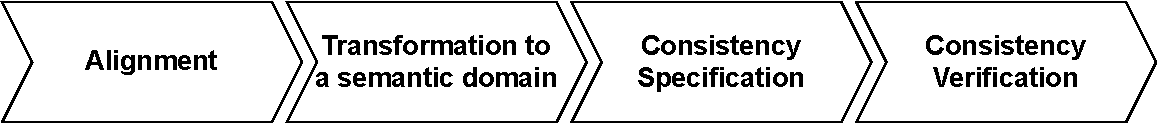
\includegraphics[width=3.4in]{methodology}
    \caption{Behavioral Consistency Management Process}
    \label{fig:consistency_process}
\end{figure}
% 1. Consistency specification
A potential consistency problem for a set of behavioral models triggers the consistency management process.
The first step of the process begins with a problem discussion and an informal problem statement.
The step concludes by formalizing the consistency problem.
To formalize the problem, one should add atomic propositions to the states of the individual models with the problem statement in mind.
Then, we can calculate the disjoint union of all atomic propositions and use this set of propositions to formalize our constraint in a temporal logic as if we had one model describing the global system.

% 2. Metamodel and model aligment
To check inter-model consistency for structural models, one defines inter-relations between models on the metamodel level and the model level to describe overlaps in information \cite{stunkelMultipleModelSynchronization2020, elhamlaouiAlignmentViewpointHeterogeneous2016}.
We propose a similar approach for behavioral models based on inter-model relations.
The inter-model relations on the metamodel level define how behavioral models can coordinate.
Thus, we call them \textit{coordinations}.
The inter-model relations on the model level should state how models interact, which leads to the composite system's behavior.
Consequently, we call them \textit{interactions}.

The second step is to define inter-model relations, i.e., coordinations and interactions.
Firstly, one has to define coordinations that align the metamodels.
For this approach to work, there must be a metamodel for each used model.
However, developing a metamodel if it is not already present is a one-time expense.
Similarly, metamodel alignment must be only done once.
In \autoref{sec:currentStatus}, we will align the metamodels for finite state machines and Petri nets.
In the future, other formalisms can be integrated similarly.
Secondly, one must align the models by defining interactions between them.
For example, the synchronization of a transition in a state machine with a transition in a Petri net could be specified.
\textit{Model alignment} is also an essential activity in the multi-model consistency management process for structural models \cite{stunkelMultipleModelSynchronization2020}.

% 3. Transformation to a semantic domain (proposes graph grammars)
The third step in the process is to transform the models into a suitable semantic domain respecting their interactions.
By including the inter-model relations in the transformation, we can deal with a heterogeneous modeling scenario compared to the original methodology in \cite{engelsMethodologySpecifyingAnalyzing2001}.
A feasible approach is to translate each model individually and then combine them according to the defined interactions.

We will use graph grammars as a behavioral formalism for the model execution (see \autoref{sec:currentStatus}) for the following reasons.
Many behavioral formalisms have been described by graph grammars, for example, state machines \cite{kuskeFormalSemanticsUML2001, varroFormalSemanticsUML2002}, Petri nets \cite{ehrigGraphGrammarsPetri2004}, the $\pi$-calculus \cite{gadducciGraphRewritingPcalculus2007}, and workflow models \cite{rutleMetamodellingApproachBehavioural2012}.
Using graph grammars, one stays on a higher level of abstraction than, for example, transition systems as a semantic domain.
This has the advantage that the state space generated by graph grammars is better understandable.
Counterexamples for consistency constraints should be easier to understand because we stay closer to the original modeling formalisms.
Being on a higher level makes it easier to implement different communication variants such as synchronous and asynchronous message passing.
In addition, structural models are formalized as graphs or graph-like structures \cite{stunkelMultipleModelSynchronization2020}, which can lead to an integration of behavioral and structural models using graph transformations in the future. 
However, the semantic domain is interchangeable if there is an interpretation for the given models and their interactions.

% 4. Consistency Verification
The fourth step in the process is concerned with verifying the specified behavioral consistency.
The semantic domain should generate a state space for the overall system that is related to the original models.
This should allow us to attach the atomic propositions from the individual models to the generated state space.
Thus, one gets a Kripke structure (state space and atomic propositions \cite{clarkeHandbookModelChecking2018}) to check behavioral constraints.
Besides checking general properties such as deadlocks, the model-specific constraints defined in step one should be checked.
We aim to reuse existing model checkers to evaluate the defined constraints on the resulting Kripke structure.

In the best case, the specification of constraints is independent of the choice of the semantic domain, such that the behavioral constraints can be checked automatically.
Generally, user input is also possible in this step if the chosen semantic domain does not precisely match the previously defined constraints.
However, this is not desirable since the semantic domain should be mostly hidden from the user.

\section{Plan for evaluation and validation}
To evaluate our methodology, we plan to implement a tool for behavioral consistency checking.
It should come with a textual \gls{dsl} for metamodel and model alignment, automatic transformations to a semantic domain, and the semantic domain's implementation, including consistency verification.
For graph grammars, one can use tools like GROOVE \cite{ghamarianModellingAnalysisUsing2012, rensinkGROOVESimulatorTool2004}, or Verigraph \cite{costaVerigraphSystemSpecification2016} to generate a state space from a graph grammar.
Especially the performance of graph grammars as a semantic domain must be critically evaluated.
If the prototype can handle artificial scenarios successfully, one can move on to industry case studies.

\section{Expected contributions}
We plan to make the following contributions:
\begin{itemize}
    \item A new methodology for behavioral consistency checking in heterogeneous cases.
    \item Metamodels and metamodel alignments for common behavioral modeling formalisms.
    \item A semantic domain for advanced behavioral consistency checking.
\end{itemize}
Besides these theoretical contributions, we plan to develop a modeling tool for metamodel and model alignment and behavioral consistency checking following the proposed methodology.

\section{Current status} \label{sec:currentStatus}
Our work on behavioral consistency has just started, such that we do not have an implementation of the following theoretical aspects yet.
So far, finite state machines and Petri nets have been considered as behavioral models/formalisms.

We will use the example models depicted in \autoref{fig:running_example} to explain the current status of our work by following the proposed methodology.
\autoref{fig:running_example} depicts three state machines, $SM^1$-$SM^3$, and a Petri net $N^1$ (ignore the cyan connections for now).
As a convention, Petri net edges have the weight one if not explicitly stated otherwise.
The state machines $SM^1$ and $SM^2$ represent two resources that can be acquired and released by the processes defined by $SM^3$ and $N^1$.
$SM^3$ acquires both resources, does some work, and then releases them, while the three processes modeled in the Petri net $N^1$ only need one of the two resources to do their work.
What each process is doing with the resources is kept abstract.
However, in practice, we often face situations in which multiple processes are competing for the same resources.

\begin{figure*}[h]
    \centering
    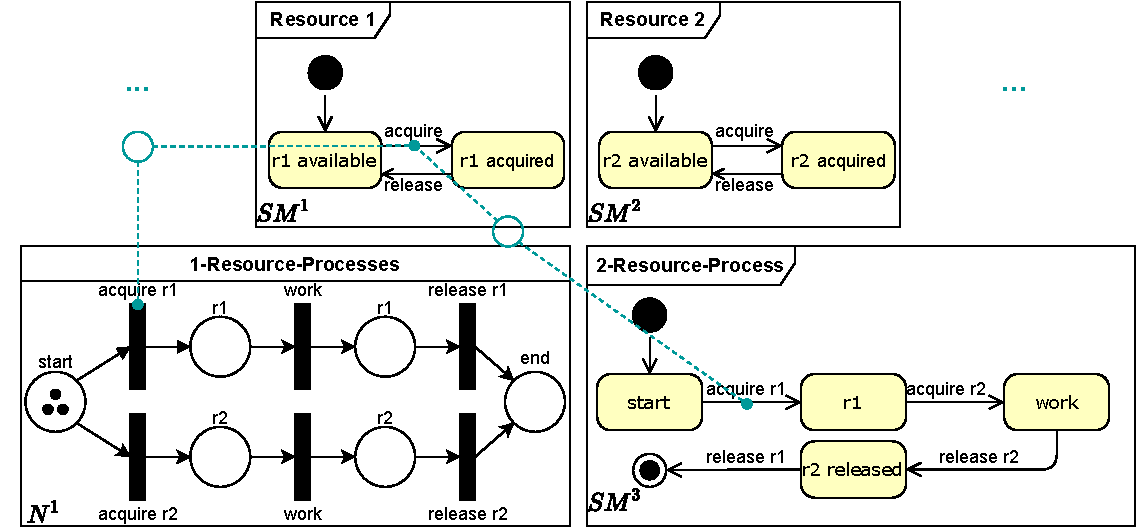
\includegraphics[width=5in]{example}
    \caption{Example models $SM^1$, $SM^2$, $SM^3$, $N^1$, and their interactions}
    \label{fig:running_example}
\end{figure*}

One could have used Petri nets to model the state machines in \autoref{fig:running_example}.
Nevertheless, we have used state machines to model most processes of the running example since the extra features of Petri nets were not needed.
In this case, the difference between a Petri net model and a state machine model for a resource is tiny, but in general, one formalism can be better suited for a given aspect of a system.

A reasonable consistency requirement for the overall system resulting from executing the models in parallel is that all processes always finish their execution.
In addition, each resource is accessed by at most one process at a time.
Thus, we formulate the following constraints:
\begin{enumerate}
    \item \textbf{Successful termination:} The state where both resources are available while $SM^3$ is in its final state and $N^1$ has three tokens in the place \textit{end} should eventually be reached.
    \item \textbf{Proper resource one access:} There can be at most one token in the places \textit{r1} while $SM^3$ is in the state \textit{start} or \textit{end}.
    If $SM^3$ is not in the state \textit{start} or \textit{end}, there must be no token in the places \textit{r1}.
    \item \textbf{Proper resource two access:} There can be at most one token in the places \textit{r2} while $SM^3$ is not in the state \textit{work}.
    If $SM^3$ is in the state \textit{work}, there must be no token in the places \textit{r2}.
\end{enumerate}

The constraints can be formalized using temporal logic by assigning appropriate atomic propositions to the mentioned states.
The first constraint can be seen as a liveness property, while the second and third constraints describe safety properties.

To check our constraints, we need to define finite state machines and Petri nets, state their respective metamodels, and align them.
After that, we can align the models of our running example depicted in \autoref{fig:running_example}.
% Model alignment for FSM's <--> Petri nets and FSM's/Petri nets <--> pi-calculus

\begin{definition}[Finite state machines] \label{def:fsm}
    A finite state machine $M=(S, \Sigma, \delta, s_0, F)$ consists of a set of states $S$, a finite alphabet $\Sigma$, a state transition relation $\delta \subseteq S \times \Sigma \times S$, an initial state $s_0 \in S$ and a set of final states $F \subseteq S$ \cite{kunzeBehaviouralModelsModelling2016}. % Def. 3.2
\end{definition}

\autoref{fig:fsm_metamodel} depicts the metamodel $M^1$ for finite state machines.
In the remainder of this paper, we will use the term state machines to refer to finite state machines.
In addition to \autoref{def:fsm}, we added names to states and state machines.
The finite alphabet $\Sigma$ is not made explicit but can be derived by the transition names of a given state machine.
The clouds in \autoref{fig:fsm_metamodel} depict concrete syntax elements inspired by \gls{uml} statecharts.
The concrete syntax elements for state machines and the one following for Petri nets are already used in \autoref{fig:running_example}.

% can be put sideways if we need the space
\begin{figure}[h]
    \centering
    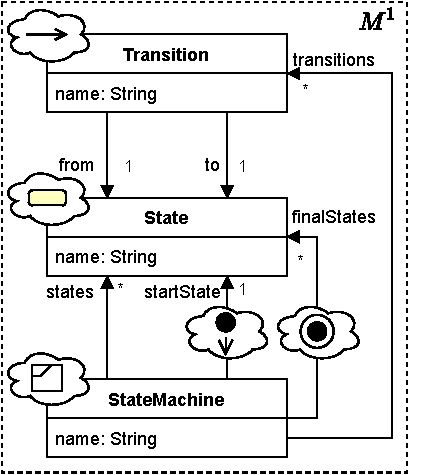
\includegraphics[width=2.3in]{state_machine_metamodel}
    \caption{Finite state machine metamodel $M^1$}
    \label{fig:fsm_metamodel}
\end{figure}

\begin{definition}[Petri net] \label{def:pn}
    A Petri net $N=(P,T,F, \omega)$ consists of a finite set of places $P$, a non-empty finite set of transitions $T$ ($T \cap P = \emptyset $), a flow relation $F \subseteq (P \times T) \cup (T \times P)$, and a weighting function $\omega: F \to \mathbb{N}$ \cite{kunzeBehaviouralModelsModelling2016}. % Def. 4.1 + 4.4 for weights
\end{definition}

\autoref{fig:petri_net_metamodel} illustrates the metamodel $M^2$ for Petri nets\footnote{Formally edges representing elements of the flow relation can have transitions or places as source and target which does not conform to \autoref{def:pn}.
We will ignore this issue for now, since we do not want to introduce constraints to the metamodel.}.
In addition to \autoref{def:pn}, places have a set of tokens since we want to model states of Petri nets, which are token distributions.
We again added names to transitions, places, edges, and the Petri net itself.
The concrete syntax for the metamodel is also given, where edge weights should be written above the arrow depicting the edge.
The default weight is one if no weight is specifically stated.

\begin{figure}[h]
    \centering
    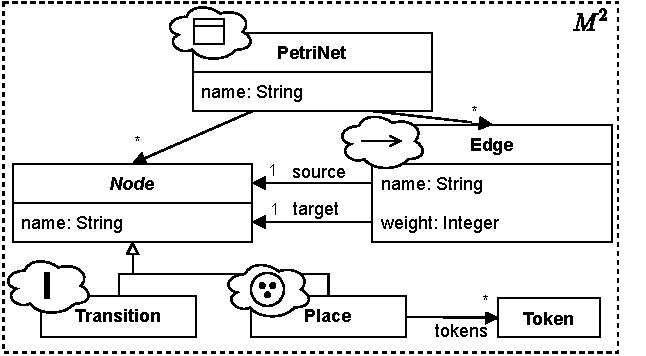
\includegraphics[width=3.4in]{petri_net_metamodel}
    \caption{Petri net metamodel $M^2$}
    \label{fig:petri_net_metamodel}
\end{figure}

Aligning the metamodels for finite state machines and Petri nets is straightforward since both formalisms rely on transitions to change the application state.
Consequently, transitions are aligned, as shown in \autoref{fig:fsm_pn_alignment}.
The inter-model relation relating the two is called synchronous communication and should be interpreted as two transitions firing simultaneously, i.e., handshaking in a semantic domain.
One could also add an inter-model relation for asynchronous communication between transitions.

\begin{figure}[h]
    \centering
    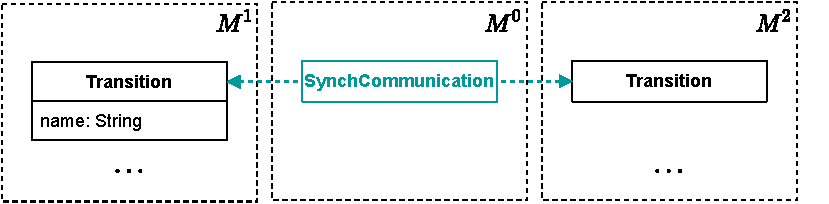
\includegraphics[width=3.48in]{fsm_pn_alignment}
    \caption{Alignment of the metamodels $M^1$ and $M^2$}
    \label{fig:fsm_pn_alignment}
\end{figure}

It is sufficient to interpret \autoref{fig:fsm_pn_alignment} as defining the existence of a set of pairs of transitions $SynchCom \subseteq \delta \times T$.
A different formalization suitable for more complex model alignment is the comprehensive system construction \cite{stunkelMultipleModelSynchronization2020}.

% Model alignment
The cyan connections in \autoref{fig:running_example} suggest the model alignment for our running example.
All \textit{acquire r1}/\textit{acquire r2} transitions are synchronized with the \textit{acquire} transition for the resource 1/2.
Formally we obtain four sets of synchronizations since we have two models synchronizing with two resources.
Aligning the state machine metamodel with itself (formally needed for the alignment of $SM^2$ and $SM^3$) is not explicitly shown but is analogous to the alignment shown in \autoref{fig:fsm_pn_alignment} for Petri nets.
The model alignment states how the models interact with each other, which is crucial for the state space generation in the chosen semantic domain.

% Transformation of FSM's, Petri-nets and maybe the pi-calculus.
We will choose graph grammars as a semantic domain for the reasons stated earlier, but one could also choose a different domain or switch in the future.
Our approach is to transform each model into a graph grammar and combine the resulting grammars to realize the defined coordination between the models.

The semantic domain of graph grammars is defined as follows.
\begin{definition}[Graph grammar] \label{def:graphGrammar}
A graph grammar $GG=(S, P)$ consists of a start graph $S$ and a set of production rules $P$ \cite{ehrigGraphGrammarsPetri2004}. 
\end{definition}
\begin{definition}[Production rule] \label{def:productionRule}
A production rule $P= L \overset{l}{\leftarrow} K \overset{r}{\to} R$ consists of graphs L, K, R, and injective graph morphisms $l: K \to L$ and $r: K \to R$ \cite{ehrigGraphGrammarsPetri2004}. 
\end{definition}

Informally speaking, elements in $R$ but not in $L$ are added by a rule, while elements in $L$ and $R$ are preserved.
A rule deletes elements that are in $L$ but not in $R$.

% Transformation Petri net
The transformation from Petri nets to graph grammars is based on the semantics defined in \cite{ehrigGraphGrammarsPetri2004}.
We assume that the token distribution in a Petri-net model $pn$ corresponds to its initial state.
Thus, the start graph is given by the graph, which only contains the places and tokens from $pn$.
Each transition is transformed to a production rule which removes tokens from the incoming places of the transition and adds tokens to the outgoing places of the transition according to the defined weights.
For the Petri net $N^1$, the resulting graph grammar will have six rules, where each rule removes one token from the previous place and adds one token to the following place.

% Transformation state machine
The initial state of a graph grammar representing a state machine is given by the graph only containing its start state.
Again, each transition is transformed to a production rule that removes the transition's source state and adds the transition's target state.
Consequently, during the execution of a state machine, the corresponding graph will always only contain the current state.

% show combined start state for the sample and the combined rule
Combining a set of graph grammars for state machines and Petri nets is given by the union of start states and the merge of production rules.
All production rules without synchronization carry over unchanged.
Every pair in a \textit{SynchCom} set leads to one rule where the three graphs of the rule are the component-wise union of the two underlying rules.

In our running example, the synchronization (cyan connection) between $SM^1$ and $N^1$ leads to the rule shown in \autoref{fig:combined_rule}.
However, since we have four synchronization sets, we also get a joint rule where \textit{acquire} of $SM^1$ synchronizes with \textit{acquire r1} in $SM^3$.
This means resource one either synchronizes with $N^1$ or $SM^3$, but never both.

\begin{figure}[h]
    \centering
    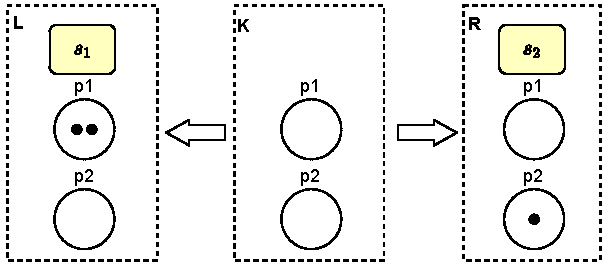
\includegraphics[width=3.4in]{combined_rule}
    \caption{Resulting rule (acquire, acquire r1) for \autoref{fig:running_example}}
    \label{fig:combined_rule}
\end{figure}

The state space generated by the final graph grammar is essentially a combination of states of the individual state spaces.
Consequently, we can carry over the atomic propositions from the individual models and even check local constraints for individual models in the global state space.
More interestingly, one can check the inter-model behavioral constraints defined earlier using the union of atomic propositions.

For our running example, we would generate the state space from the previously obtained graph grammar and attach the set of defined atomic propositions.
Afterwards, we can check the consistency constraints formulated in the first step of the consistency management process.
Eventual counterexamples to our constraints should be understandable since the graph grammar directly operates on instances of the defined metamodels.
We checked the behavioral consistency for our running example using Groove\footnote{\url{https://github.com/timKraeuter/MODELS-2021-Doctoral-Symposium/tree/main/example_implementation_groove}.}.

% Timeline
We plan to finish the theoretical foundations in the next few months by defining executable algorithms for the transformation of state machines and Petri nets to the semantic domain.
Afterwards, during the last month of this year, we plan to implement a prototype to automate the transformation to the semantic domain, including consistency verification.
In parallel, we integrate the $\pi$-calculus in the semantics domain of graph grammars inspired by \cite{gadducciGraphRewritingPcalculus2007}.
Other popular behavioral models such as \gls{uml} activity diagrams and \gls{bpmn} models should be investigated in the near future. 


\section{Conclusion}
We proposed a methodology for handling heterogeneous behavioral model consistency.
To the best of our knowledge, current approaches only offer limited consistency checking in a heterogeneous scenario.
To cope with heterogeneity, metamodel and model alignment are proposed inspired by the model alignment of structural models.

Furthermore, we have proposed graph grammars as a suitable semantic domain for behavioral consistency checking.
Finite state machines and Petri nets, as two fundamental behavioral formalisms, have been encoded in the graph grammar domain.
Their metamodels have been aligned, and the intended synchronization semantics were highlighted using a running example. 

The current work develops a solid formal foundation for behavioral consistency checking but has to be expanded, implemented, and tried in practice.
The performance of the approach and its applicability to real-world scenarios must be investigated.

Possible future work is adding asynchronous communication, synchronizing multiple Petri net transitions with one state machine transition, or synchronizing more than two transitions from different models with each other.
In addition, more behavioral models must be included in the future to allow for more heterogeneity.
One could also aim to include continuous-time models for more diverse modeling scenarios.

\section*{Acknowledgment}
The author would like to thank Harald König, Adrian Rutle, and Yngve Lamo for fruitful discussions about the topic.

\bibliographystyle{IEEEtran}
\bibliography{bib}

\end{document}


